\documentclass[a4paper]{article}

\usepackage{fullpage} % Package to use full page
\usepackage{parskip} % Package to tweak paragraph skipping
\usepackage{tikz} % Package for drawing
\usepackage{amsmath}
\usepackage{amssymb}
\usepackage{hyperref}
\usepackage{multirow}
\usepackage{booktabs}


\title{Programming Assignment 2 : Strassen's}
\author{HUIDS: 90978217 AND 10978211}
\date{03/24/2017}

\begin{document}

\maketitle

\section{Overview}
In this programming assignment, we implement an optimized version of Strassen's algorithm to multiply two $n$ by $n$ matrices. Because Strassen's is slower than conventional matrix multiplication for small matrices, our algorithm uses Strassen's for matrices down to a certain threshold size $n_0$, at which point which we utilize standard matrix multiplication. We find $n_0$ both analytically and experimentally. The results from our studies are presented in this report.

Our code may be run by executing the following commands in the terminal:
\begin{verbatim}
$ make
$ ./strassen <verbosity> <dimension> <inputfile>
\end{verbatim}
where \texttt{verbosity} specifies the verbosity of the output (0 for the minimal output specified in the specs, 1 for a more detailed output).

\section{Method}
\subsection{Algorithm}
We use an optimized version of Strassen's algorithm to multiply two size $n$ matrices $A$ and $B$, where our algorithm switches to standard matrix multiplication for matrices of size $n_0$. Note that because Strassen's decomposes each larger matrix multiplication into smaller multiplications of blocks of size $n/2$, we want our starting matrices to be of size $n_02^k$, where $k$ is the smallest possible integer such that $n_02^k > n$. To achieve this, we statically pad the bottom and right of our starting matrices with 0s until they reach the desired size. When our algorithm is finished, we remove this extra padding of 0s to obtain our final output matrix.

Once we have correctly-sized starting matrices, we recursively call Strassen's algorithm on $A$ and $B$ until the recursive calls work on matrices of size $n_0$, at which point we switch to standard matrix multiplication. On inputs of size $k$, Strassen's requires us at each recursive level to store seven temporary matrix subproducts of size $k/2$ and add different combinations of these subproducts up to achieve our final output matrix $C$. To optimize for space and avoid storing each of these subproducts, we store most of the temporary subproducts in the output matrix $C$, conducting our computations in an order such that we only require two temporary storage matrices of size $k/2$ each. The order of computations, which we obtained from [CITE HERE: https://www.cise.ufl.edu/~sahni/papers/strassen.pdf] is as follows:
\begin{center}
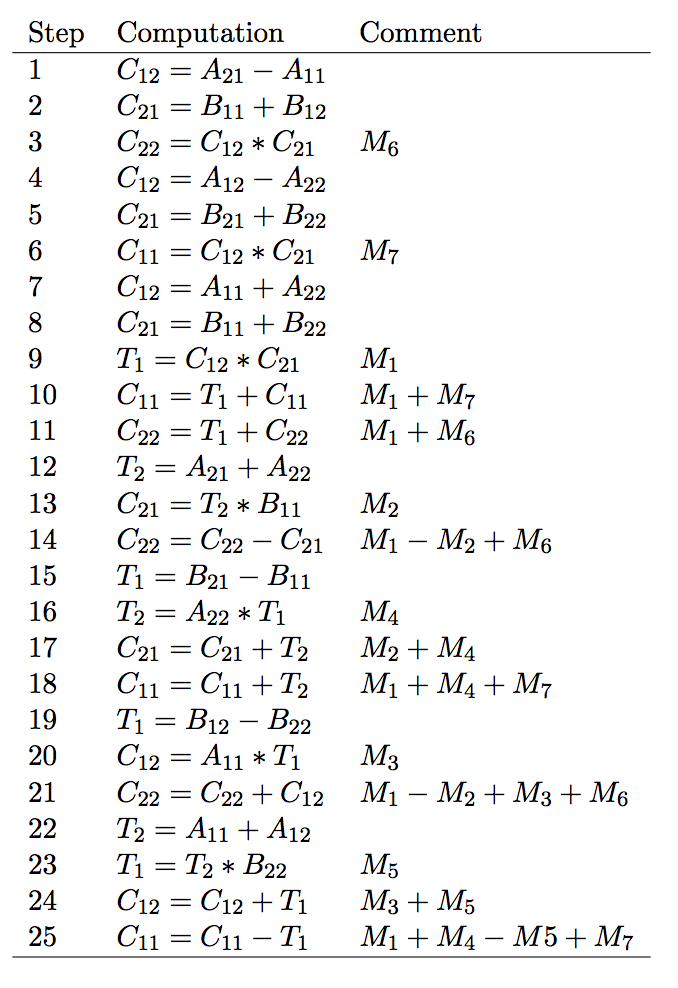
\includegraphics[width=3in]{computations.png}
\end{center}

Once Strassen's decomposes into size $n_0$ matrices, we implement an optimized version of standard matrix multiplication... @MELLY BLAH BLAH OPTIMIZED CACHING SHIT

When considering how to pad our matrices to obtain the appropriate matrices, we also considered dynamic padding. Dynamic padding works by adding an extra row and column of padding only if the matrices being multiplied have an odd dimension, and then removing these extra 0s after the two matrices are multiplied. This method mitigates the costs of multiplying unnecessarily large matrices (a possible concern in static padding), and is a possible consideration for future work.

\textbf{Runtime.} As discussed in class, the standard matrix conventional matrix multiplication algorithm runs in $\Theta(n^3)$, while Strassen's runs in $\Theta(n^{log_27})$.



\subsection{Implementation}
Our eager implementation of Prim's algorithm uses two main classes:

\begin{itemize}
	\item \texttt{Vertex}: Represents a vertex in the complete graph. The main attributes are:
	\begin{itemize}
		\item \texttt{minimum-distance}: Minimum distance (edge weight) connecting this vertex to the current MST. Whenever a new vertex $v$ is added to the MST, each edge leaving $v$ is relaxed; the \texttt{minimum-distance} of neighbor $u$ is updated only if the weight of edge$(v, u_i)$ is smaller than the current minimum distance. This value fixes once a vertex is added to the MST, and allows us to calculate the final weight of the MST.
		\item \texttt{coordinates}: An array holding the vertex's coordinates, if applicable. Allows us to calculate the edge weights for Euclidean graphs.
		\item \texttt{key}: Unique integer key between 0 (inclusive) and the number of points (exclusive) associated with each vertex. Allows us to reference vertices in the priority queue.
	\end{itemize}
	Note that \texttt{Vertex} does not keep an adjacency list in memory. Because we are only generating MST's on complete graphs, where all possible edges between $n$ points exist, we can simply iterate through all entries in the current priority queue (which is initialized to all vertices) to touch all neighbors of a vertex not already in the MST. This is correct because we always maintain the invariant that the priority queue contains only those vertices not already in the MST.
	
	\item \texttt{RandMST}: Represents a MST on a complete graph. The main attributes are: 
	\begin{itemize}
		\item \texttt{graph}: An array holding all $n$ vertices in the graph, where the vertex with key $i$ is in position $i$.
		\item \texttt{priority-queue}: A binary heap implementation of the priority queue; the queue is an integer array containing vertex keys, where the first element is the top of the heap. We use a integer variable to track the ``end'' of the queue, and never modify the size of the array.
	\end{itemize}
\end{itemize}

Additionally, we make use of a general \texttt{Experiment} object, which is passed into the constructor for Random MST's. The \texttt{Experiment} object has methods for calculating the weight of any given edge, and for creating a new graph with random vertices, allowing us to generalize our code for many types of random spanning trees. 

\section{Results and Discussion}

\subsection{Analytically determining threshold}
We analytically determine a crude approximation to the cross-over point $n_0$ at which the standard matrix multiplication algorithm runs more quickly than normal Strassen's.

First, we note that the standard matrix multiplication algorithm requires $n$ multiplications and $n-1$ additions for each of the $n^2$ entries in the output. Thus:
$$R(n) = n^2(n + (n-1)) = 2n^3 - n^2$$

We note that normal Strassen's matrix multiplication algorithm decomposes each input matrix of size $n$ into seven multiplications of submatrices of size $n/2$, along with 18 additions of matrices of size $n/2$ (see table above). Thus, we can describe normal Strassen's via the following recurrence equation: 
$$S(n) = 7S(n/2) + 18(n/2)^2$$

We note that our optimized version of Strassen's uses our conventional matrix multiplication algorithm once the recursive calls reach inputs of size $n_0$. Thus, at this point:
\begin{align*}
R(n) &= 7R(n/2) + 18(n/2)^2 \\
2n^3-n^2 &= 2(n/2)^3 - (n/2)^2 + 18(n/2)^2
\end{align*}
Solving for $n$ gives us $n=15$. BLAHBLAH


\subsection{Experimentally determining threshold}



Our code runs reasonably quickly, taking less than 1 second on average to generate a MST for random graphs of size $n\leq2^{13}$, less than 15 seconds for $n\leq 2^{15}$, around 1.5 minutes for $n=2^{16}$, and around 5.5 minutes for the maximal graph size we tested, $n=2^{17}$. Note that our main time consumption stems from the $O(E)$ calls to ``decrease-key'' on our binary heap. With this in mind, using a Fibonacci heap, which has constant amortized time decrease-key operations, could significantly speed up our implementation to run in $O(n\log n)$ time. This is a direction for future work.

\newpage
After running our algorithm on MSTs with vertices $n=2^7, 2^8, ..., 2^{17}$, we obtained the following results for average MST weight:

\begin{table}[htbp]
  \centering
    \begin{tabular}{cr|rrrr}
          & \multicolumn{1}{r}{} & \multicolumn{4}{c}{\textbf{Dimension}} \\
          &       & \textbf{0} & \textbf{2} & \textbf{3} & \textbf{4} \\
\cmidrule{2-6}    \multirow{11}[1]{*}{\textbf{$\log_2n$}} & \textbf{7} & 1.113 & 7.716 & 17.833 & 28.518 \\
          & \textbf{8} & 1.181 & 10.797 & 27.597 & 46.919 \\
          & \textbf{9} & 1.188 & 14.852 & 43.057 & 78.282 \\
          & \textbf{10} & 1.190 & 21.093 & 67.795 & 130.567 \\
          & \textbf{11} & 1.197 & 29.657 & 107.295 & 216.398 \\
          & \textbf{12} & 1.200 & 41.828 & 169.348 & 360.653 \\
          & \textbf{13} & 1.201 & 58.878 & 266.873 & 603.351 \\
          & \textbf{14} & 1.201 & 83.074 & 422.195 & 1009.779 \\
          & \textbf{15} & 1.201 & 117.552 & 668.605 & 1686.334 \\
          & \textbf{16} & 1.204 & 166.121 & 1058.731 & 2827.767 \\
          & \textbf{17} & 1.202 & 234.581 & 1677.107 & 4740.367 \\
    \end{tabular}%
  \caption{Average MST weights for various values of $\log_2n$ and dimension.}
  \label{tab:addlabel}%
\end{table}%

Examining these results, we make a few preliminary observations: The average minimal tree weight for the random-weight graphs appears to converge towards a constant, leveling off around $f(n) = 1.203$. On the other hand, the average tree weight for Euclidean distance-weighted graphs appears to grow at a decreasing rate, indicating that the second derivative of the function is negative. A reasonable guess for the function is something of the form $f(n) = cn^k$, where $c>0$ (all tree weights must be strictly positive) and $f''(n) = ck(k-1)n^{k-2} < 0$. Solving for values of $k$ that satisfy the inequality for all $n>0$ yields $0<k<1$. Thus, our initial guess for $f(n)$ is a power function with exponent between 0 and 1, exclusive. Performing linear least-squares regression on the log of the data in R confirms these observations, yielding good fits for the data, and showing that the optimal value of $k$ appears to be different for different dimensions. Based on the fits, we guess that $k\approx \frac{d}{d-1}$, where $d$ is the dimension.

Our final estimates for $f(n)$ using non-linear least squares analysis for the family of power functions $cn^{\frac{d-1}{d}}$ are presented below:


The growth rate for Euclidean distance-weighted graphs is not surprising. First, we note that this function's second derivative is negative, indicating that greater values of $n$ correspond to a lesser increase in $f(n)$. This makes sense, because increasing the number of vertices while limiting the coordinates of each vertex to a unit square/cube/hypercube results in vertices that are clustered more closely together, decreasing the impact of any additional vertices on total MST weight. Thus, a increase in $n$ will not result in an equally proportional increase in $f(n)$, since new vertices are likely to be closer together to existing vertices.

Second, we also note that as the numbers of dimensions increases, the growth rate of $f(n)$ approaches $O(n)$. Again, this makes sense, because increasing the number of dimensions that each vertex has access to decreases the aforementioned clustering effect; that is, adding additional vertices are less likely to result in a graph that is tightly clustered, since these extra vertices are more likely to be "farther" away from existing vertices.

For the random weights case, we simply model the relationship with a constant, because we noted that values of $f(n)$ appeared to converge to a value of around 1.203 as $n$ increased. The data are plotted below, along with a line representing the average value of $f(n)$.


Intuitively, this result is not surprising, because increasing $n$ here simply adds vertices to a cluster of extremely ``closely-connected'' nodes (if we visualize edge weight as distance), such that adding additional vertices will have less and less impact on the total minimum spanning tree weight as the size of the graph increases (since any additional vertices will exist within this dense ball).

\end{document}